% 12pt: grandezza carattere
% a4paper: formato a4
% openright: apre i capitoli a destra
% twoside: serve per fare un
% documento fronteretro
% report: stile tesi (oppure book)
\documentclass[12pt,a4paper,openright,twoside]{report}

%libreria per scrivere in italiano
\usepackage[italian]{babel}

% libreria per accettare i caratteri
% digitati da tastiera come ?
% si può usare anche
% \usepackage[T1]{fontenc}
% però con questa libreria
% il tempo di compilazione
% aumenta
\usepackage[latin1]{inputenc}

% libreria per impostare il documento
\usepackage{fancyhdr}

% libreria per avere l'indentazione all'inizio dei capitoli, ...
\usepackage{indentfirst}

%libreria per mostrare le etichette
%\usepackage{showkeys}

% libreria per inserire grafici
\usepackage{graphicx}

% libreria per utilizzare font particolari ad esempio \textsc{}
\usepackage{newlfont}

% librerie matematiche
\usepackage{amssymb}
\usepackage{amsmath}
\usepackage{latexsym}
\usepackage{amsthm}

% librerie per mostrare il codice sorgente
\usepackage{listings, xcolor}
\renewcommand{\lstlistingname}{Codice sorgente}
\renewcommand{\lstlistlistingname}{Codici sorgenti}
% impostano i margini
\oddsidemargin=30pt
\evensidemargin=20pt

% serve per la sillabazione: tra parentesi vanno inserite come nell'esempio le parole
% che latex non riesce a tagliare nel modo giusto andando a capo.
\hyphenation{sil-la-ba-zio-ne pa-ren-te-si}

% comandi per l'impostazione della pagina, vedi il manuale della libreria fancyhdr per ulteriori delucidazioni
\pagestyle{fancy}\addtolength{\headwidth}{20pt}
\renewcommand{\chaptermark}[1]{\markboth{\thechapter.\ #1}{}}
\renewcommand{\sectionmark}[1]{\markright{\thesection \ #1}{}}
\rhead[\fancyplain{}{\bfseries\leftmark}]{\fancyplain{}{\bfseries\thepage}}
\cfoot{}

%comando per impostare l'interlinea
\linespread{1.3}

\begin{document}

\begin{titlepage}
% crea un ambiente libero da vincoli di margini e grandezza caratteri: si pu\`o modificare
% quello che si vuole, tanto fuori da questo ambiente tutto viene ristabilito

% elimina il numero della pagina
\thispagestyle{empty}

% imposta il margina superiore a 6.5cm
\topmargin=6.5cm

% incolonna la scrittura a destra
\raggedleft

% aumenta la grandezza del carattere a 14pt
\large

% emfatizza (corsivo) il carattere
\em

%\ldots lascia tre puntini
%\ldots

% va in una pagina nuova
\newpage

% non numera l'ultima pagina sinistra
\clearpage{\pagestyle{empty}\cleardoublepage}
\end{titlepage}

\pagenumbering{roman} % serve per mettere i numeri romani
\chapter*{Introduzione} % crea l'introduzione (un capitolo non numerato)

% imposta l'intestazione di pagina
\rhead[\fancyplain{}{\bfseries INTRODUZIONE}]{\fancyplain{}{\bfseries\thepage}}
\lhead[\fancyplain{}{\bfseries\thepage}]{\fancyplain{}{\bfseries INTRODUZIONE}}

% aggiunge la voce Introduzione nell'indice
\addcontentsline{toc}{chapter}{Introduzione}
% \ldots
Questo lavoro ha l'obiettivo di implementare sul simulatore Alchemist il modello ad agenti.

Alchemist \`e un meta-simulatore estendibile, ispirato alla chimica stocastica e adatto al calcolo pervasivo e ai sistemi distribuiti. Fornisce un meta-modello flessibile, sul quale gli sviluppatori legano le proprie astrazioni, realizzando un'incarnazione.

Il modello ad agenti a cui si fa riferimento \`e quello BDI (Beliefs, Desires, Intentions) che \`e ispirato al modello del comportamento umano.


% non numera l'ultima pagina sinistra
\clearpage{\pagestyle{empty}\cleardoublepage}

%crea l'indice
\tableofcontents

% imposta l'intestazione di pagina
\rhead[\fancyplain{}{\bfseries\leftmark}]{\fancyplain{}{\bfseries\thepage}}
\lhead[\fancyplain{}{\bfseries\thepage}]{\fancyplain{}{\bfseries INDICE}}

% non numera l'ultima pagina sinistra
\clearpage{\pagestyle{empty}\cleardoublepage}

% crea l'elenco delle figure
\listoffigures

% non numera l'ultima pagina sinistra
\clearpage{\pagestyle{empty}\cleardoublepage}

% crea l'elenco delle tabelle
%\listoftables

% non numera l'ultima pagina sinistra
\clearpage{\pagestyle{empty}\cleardoublepage}

%% % crea l'elenco dei codici sorgenti
 \lstlistoflistings
%%
%% % non numera l'ultima pagina sinistra
%% \clearpage{\pagestyle{empty}\cleardoublepage}

%-%-%-%-%-%-%-%-%-%-%-%-%-%-%-%-%-%-%-%-%-%-%-%-%-%-%-%-%-%-%-%-%-%-%-%-%-%-%-%-
\chapter{Alchemist}
% imposta l'intestazione di pagina
\lhead[\fancyplain{}{\bfseries\thepage}]{\fancyplain{}{\bfseries\rightmark}}
% mette i numeri arabi
\pagenumbering{arabic}
Alchemist fornisce un ambiente di simulazione sul quale \`e possibile sviluppare nuove incarnazioni, ovvero nuove definizioni di modelli sviluppati su di esso.

%++-++-++-++-++-++-++-++-++-++-++-++-++-++-++-++-++-++-++-++-++-++-++-++-++-++-
\section{Il meta-modello}
Il meta-modello di Alchemist pu\`o essere compreso con la figura \ref{fig:alchemistModel}.
%crea l'ambiente figura;
\begin{figure}[h] % [h] sta per here, cioè la figura va qui
\begin{center} % centra nel mezzo della pagina la figura
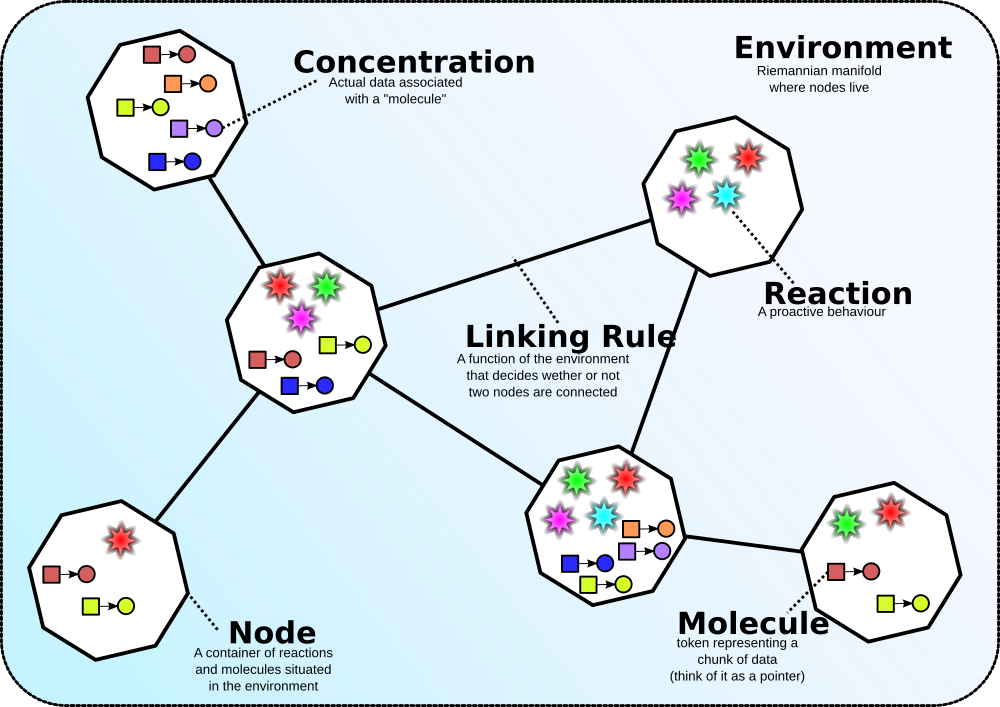
\includegraphics[width=12.5cm]{images/model.png} % inserisce una figura larga 12.5cm
% inserisce la legenda ed etichetta la figura con \label{fig:prima}
\caption[Illustrazione meta-modello di Alchemist]{Illustrazione meta-modello di Alchemist} \label{fig:alchemistModel}
\end{center}
\end{figure}

L'\textbf{\textit{Environment}} \`e l'astrazione dello spazio ed \`e anche l'entit\`a pi\`u esterna che funge da contenitore per i nodi. Conosce la posizione di ogni nodo nello spazio ed \`e quindi in grado di fornire la distanza tra due di essi e ne permette inoltre lo spostamento.

\`E detta \textbf{\textit{Linking rule}} una funzione dello stato corrente dell'environemnt che associa ad ogni nodo un \textbf{\textit{Vicinato}}, il quale \`e un entit\`a composta da un nodo centrale e da un set di nodi vicini.

Un \textbf{\textit{Nodo}} \`e un contenitore di molecole e reazioni che \`e posizionato all'interno di un environment.

La \textbf{\textit{Molecola}} \`e il nome di un dato, paragonabile a quello che rappresenta il nome di una variabile per i linguaggi imperativi.
Il valore da associare ad una molecola \`e detto \textbf{\textit{Concentrazione}}.

%crea l'ambiente figura;
\begin{figure}[h] % [h] sta per here, cioè la figura va qui
\begin{center} % centra nel mezzo della pagina la figura
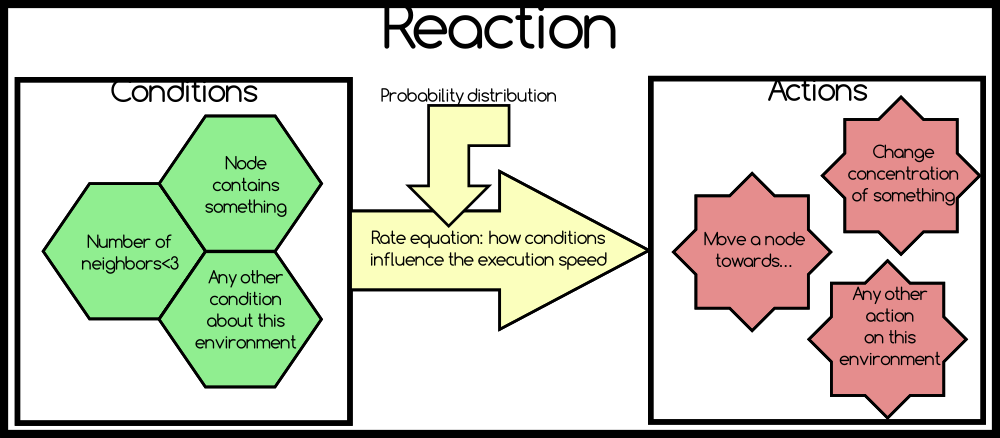
\includegraphics[width=14cm]{images/reaction.png} % inserisce una figura larga 12.5cm
% inserisce la legenda ed etichetta la figura con \label{fig:prima}
\caption[Illustrazione modello reazione di Alchemist]{Illustrazione modello reazione di Alchemist} \label{fig:alchemistReaction}
\end{center}
\end{figure}

Una \textbf{\textit{Reazione}} \`e un qualsiasi evento che pu\`o cambiare lo stato dell'environment ed \`e definita tramite una distribuzione temporale, una lista di condizioni e una o pi\`u azioni.
\\La frequenza con cui avvengono dipende da:
\begin{itemize}
\item un parametro statico di frequenza;
\item il valore di ogni condizione;
\item un'equazione di frequenza che combina il parametro statico e il valore delle condizioni restituendo la frequenza istantanea;
\item una distribuzione temporale.
\end{itemize}
Ogni nodo contiene un set di reazioni che pu\`o essere anche vuoto.

Per comprendere meglio il meccanismo di una reazione si pu\`o osservare la figura \ref{fig:alchemistReaction}.

Una \textbf{\textit{Condizione}} \`e una funzione che prende come input l'environment corrente e restituisce come output un booleano e un numero. Se la condizione non si verifica, le azioni associate a quella reazione non saranno eseguite. In relazione a parametri di configurazione e alla distribuzione temporale, una condizione potrebbe influire sulla velocit\`a della reazione.

La \textbf{\textit{Distribuzione temporale}} indica il numero di eventi che si verificano successivamente ed indipendentemente in un dato intervallo di tempo.

Un'\textbf{\textit{Azione}} \`e la definizione di una serie di operazioni che modellano un cambiamento nel nodo o nell'environment.

In Alchemist un'incarnazione \`e un'istanza concreta del meta-modello appena descritta e che implementa una serie di componenti base come: la definizione di una molecola e del tipo di dati della concentrazione, un set di condizioni, le azioni e le reazioni. Incarnazioni diverse possono modellare universi completamente differenti.

%++-++-++-++-++-++-++-++-++-++-++-++-++-++-++-++-++-++-++-++-++-++-++-++-++-++-
\section{Scrivere una simulazione}
% style for general source code
\lstset{
  numberstyle=\footnotesize\color{black},
  basicstyle=\ttfamily,
  breakatwhitespace=false,
  breaklines=true,
  captionpos=b,
  keepspaces=true,
  numbers=left,
  numbersep=0pt,
  showspaces=false,
  showstringspaces=false,
  showtabs=false,
  tabsize=2,
  frame=tb
  %label=incarnationYAML,
  %caption={First verbatim}
  %language=Java
  %escapeinside={(*@}{@*)}
}
Il linguaggio da utilizzare per scrivere le simulazioni in Alchemist \`e YAML e quello che il parser del simulatore si aspetta in input \`e una mappa YAML.
\\
Nei prossimi paragrafi verr\`a mostrato quali sezioni si possono inserire e come utilizzarle per creare la simulazione che si vuole realizzare.

La sezione \textbf{incarnation} \`e obbligatoria. Il parser YAML si aspetta una stringa che rappresenta il nome dell'incarnazione da utilizzare per la simulazione.
\medskip
\begin{lstlisting}[firstnumber=last,caption={Incarnazione}]
  incarnation: agent
\end{lstlisting}

Nel resto della sezione, il valore associato alla chiave 'type' fa riferimento al nome di una classe. Se il nome passato non \`e completo, ovvero non \`e comprensivo del percorso fino alla classe, Alchemist provveder\`a a cercare la classe tra i packages.

Per dichiarare variabili che poi potranno essere richiamate all'interno del file di configurazione della simulazione si pu\`o procedere in questo modo.
\medskip
\begin{lstlisting}[firstnumber=last,caption={Variabili simulazione}]
  variables:
    myVar: &myVar
      par1: 0
      par2: "string"
    mySecondVar: &myVar2
      par: "value"
\end{lstlisting}

Utilizzando la keyword \textbf{environment} si pu\`o scegliere quale definizione di ambiente utilizzare per la simulazione.
\medskip
\begin{lstlisting}[firstnumber=last,caption={Environment}]
  environment:
    type: OSMEnvironment
    parameters: [/maps/foo.pbf]
\end{lstlisting}
Questo parametro \`e opzionale e di default \`e uno spazio continuo bidimensionale: ometterlo equivale a scrivere la seguente configurazione.
\medskip
\begin{lstlisting}[firstnumber=last,caption={Default environment}]
  environment:
    type: Continuous2DEnvironment
\end{lstlisting}

La keyword \textbf{positions} consente di specificare il tipo delle coordinate della simulazione. La psizione riflette lo spazio fisico: per esempio non si potr\`a utilizzare la distanza \textit{Continuous2DEuclidean} se si considera la mappa di una citt\`a visto che dati due punti A e B, nel mondo reale la distanza AB \`e diversa da quella BA.
\medskip
\begin{lstlisting}[firstnumber=last,caption={Default environment}]
  positions:
    type: LatLongPosition
\end{lstlisting}

I collegamenti tra i nodi che verranno utilizzati nella simulazione sono specificati nella sezione \textbf{network-model}. Un esempio per la costruzione di collegamenti \`e il seguente.
\medskip
\begin{lstlisting}[firstnumber=last,caption={Funzione linking-rule}]
  network-model:
    type: EuclideanDistance
    parameters: [10]
\end{lstlisting}
Anche questo \`e un parametro opzionale e di default non ci sono collegamenti, ovvero i nodi nell'environemnt non sono collegati, ed \`e descritto con il seguente formalismo.
\medskip
\begin{lstlisting}[firstnumber=last,caption={Default linking-rule}]
  network-model:
    type: NoLinks
\end{lstlisting}

Il posizionamento dei nodi viene gestito dalla sezione \textbf{displacements}. Questa sezione pu\`o contenere uno o pi\`u definizioni di disposizioni per i nodi.
Il parametro 'in' definisce la geometria all'interno del quale verranno disposti i nodi, utilizzando ad esempio punti o figure come cerchi o rettangoli, mentre il parametro 'programs' definisce le reazioni da associare ad ogni nodo di quella certa disposizione.
\\
Esempi di classi utilizzabili nel parametro 'in' sono Point e Circle.
La classe Circle necessita di quattro parametri, da passare nel seguente ordine: il numero di nodi da disporre, la coordinata x del centro, la coordinata y del centro, il raggio del cerchio. Per la classe Point \`e sufficiente fornire in ordine la coordinata x e la coordinata y.

Il parametro 'programs' rappresenta le reazioni da associare ai nodi ed accetta una lista di reazioni, le quali a loro volta sono formate da una lista di parametri. Un'esempio di definizione di una reazione \`e utilizzando 'time-distribution' (valore utilizzato per settare la freqeunza) e 'program' (parametro che viene passato alla creazione della reazione e che pu\`o essere utilizzato per istanziare condizioni e azioni).
Un'esempio di displacements \`e il seguente.
\medskip
\begin{lstlisting}[firstnumber=last,caption={Disposizione nodi e reazioni associate}]
  displacements:
    - in: {type: Circle, parameters: [5,0,0,2]}
      programs:
      -
        - time-distribution: 1
          program: "reactionParam"
        - time-distribution: 2
          program: "doSomethingParam"
    - in: {type: Point, parameters: [1,1]}
      programs:
      -
        - time-distribution: 1
          program: "pointReactionParam"
\end{lstlisting}


%-%-%-%-%-%-%-%-%-%-%-%-%-%-%-%-%-%-%-%-%-%-%-%-%-%-%-%-%-%-%-%-%-%-%-%-%-%-%-%-
\chapter{Agenti}
% imposta l'intestazione di pagina
\lhead[\fancyplain{}{\bfseries\thepage}]{\fancyplain{}{\bfseries\rightmark}}

Un'agente \`e un entit\`a che agisce in modo autonomo e continuo in uno spazio condiviso con altri agenti. Le caratteristiche principali di un agente sono: autonomia, proattivit\`a e reattivit\`a. Gli agenti sono formati da un nome, che \`e una caratteristica statica, e da componenti dinamici come lo stato.

%++-++-++-++-++-++-++-++-++-++-++-++-++-++-++-++-++-++-++-++-++-++-++-++-++-++-
\section{Agenti BDI}
Gli agenti BDI forniscono un meccanismo per separare le attivit\`a di selezione di un piano fra quelli presenti nella sua teoria dall'esecuzione del piano attivo, permettendo di bilanciare il tempo speso nella scelta del piano e quello per eseguirlo.

I \textbf{\textit{Beliefs}} sono informazioni dello stato dell'agente, ovvero ci\`o che l'agente sa del mondo (di se stesso e degli altri agenti), e possono comprendere regole di inferenza per permettere l'aggiunta di nuovi beliefs. L'insieme dei belief di un agente \`e detto 'belief base' o 'belief set' e si pu\`o modificare nel tempo.

I \textbf{\textit{Desires}} sono tutti i possibili piani che l'agente potrebbe eseguire. Rappresentano gli obiettivi o le situazioni che l'agente vorrebbe realizzare o portare a termine. I \textbf{goals} sono desires che l'agente persegue attivamente: per questo motivo, in generale, i piani desiderabili possono non essere coerenti tra loro mentre i goals \`e bene che lo siano.

Le \textbf{\textit{Intentions}} sono piani a cui l'agente ha deciso di lavorare o a cui sta gi\`a lavorando. I piani sono sequenze di azioni che un agente pu\`o eseguire per raggiungere una intention. I piani possono contenerne altri al loro interno.

Gli \textbf{\textit{Eventi}} innescano le attivit\`a reattive degli agenti il cui risultato pu\`o essere l'aggiornamento dei beliefs, la chiamata ad altri piani o la modifica di goals.


%++-++-++-++-++-++-++-++-++-++-++-++-++-++-++-++-++-++-++-++-++-++-++-++-++-++-
\section{Ciclo di ragionamento}
Il ciclo di ragionamento, descritto in figura \ref{fig:reasoningCicle}, \`e il modo in cui l'agente prende le sue decisioni e mette in pratica le azioni.

In particolare, questo ciclo di ragionamento descrive quello per gli agenti implementati in Jason.

%crea l'ambiente figura;
\begin{figure}[h] % [h] sta per here, cioè la figura va qui
\begin{center} % centra nel mezzo della pagina la figura
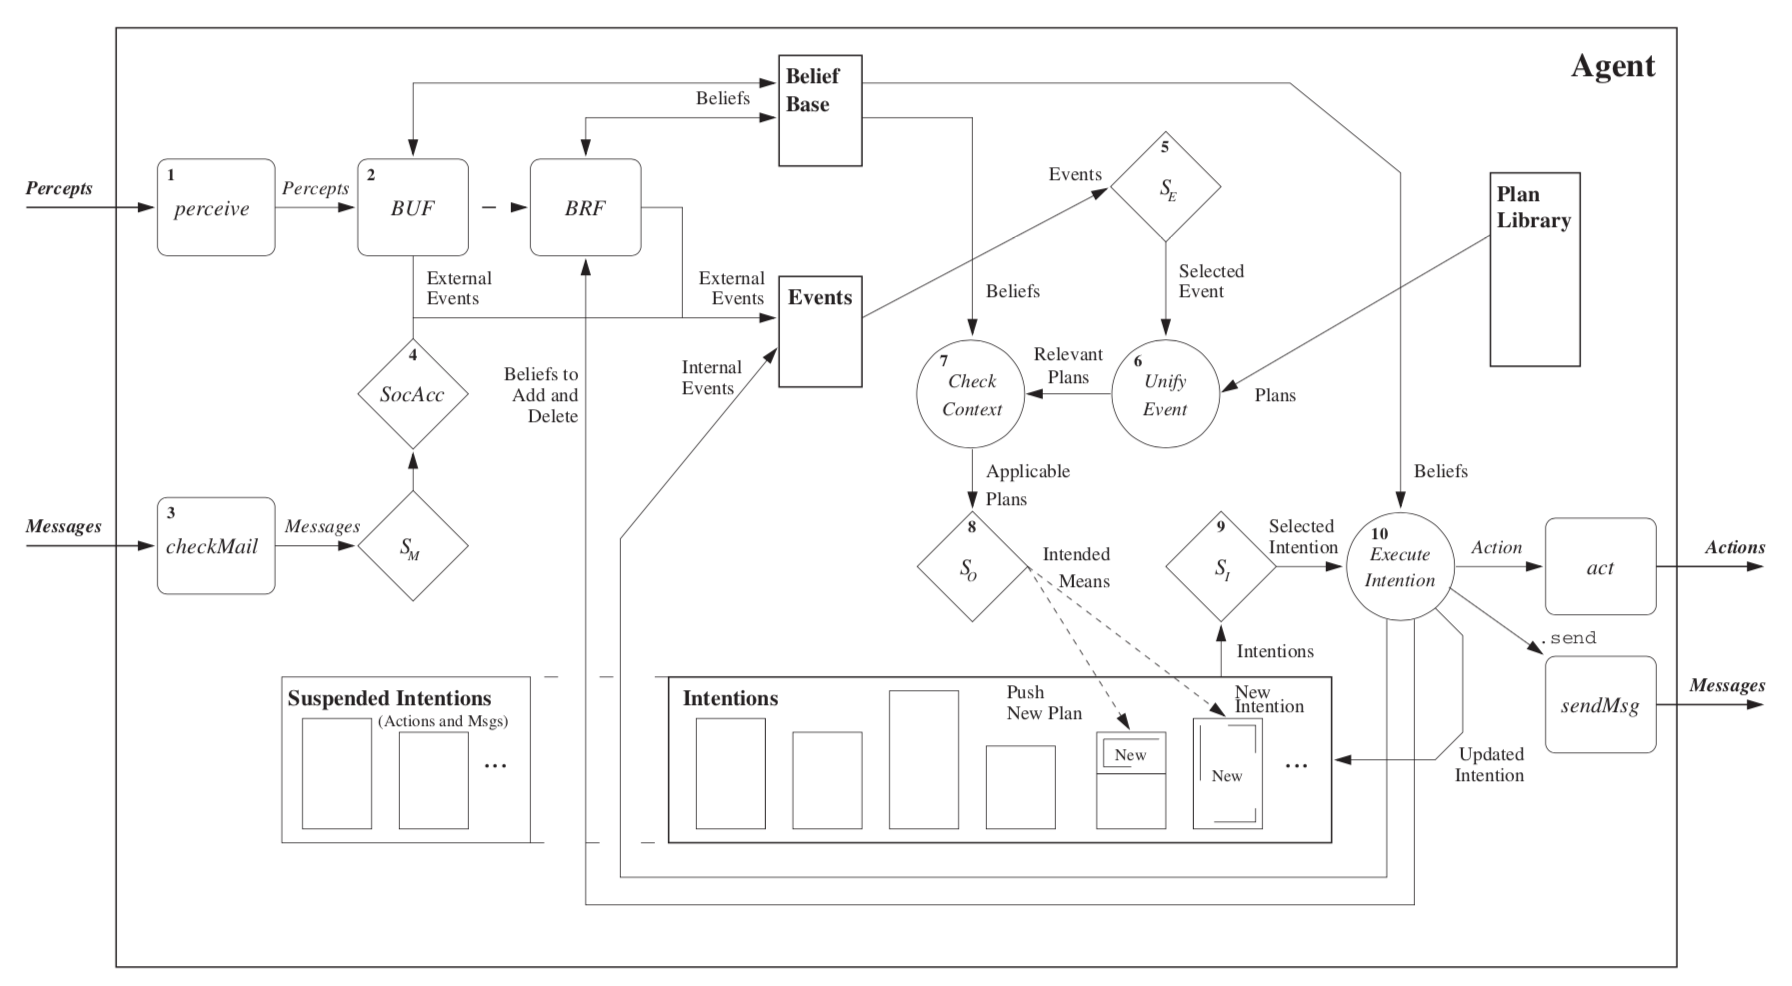
\includegraphics[width=16cm]{images/reasoningCicle.png} % inserisce una figura larga 12.5cm
% inserisce la legenda ed etichetta la figura con \label{fig:prima}
\caption[Ciclo di ragionamento di un agente]{Ciclo di ragionamento di un agente} \label{fig:reasoningCicle}
\end{center}
\end{figure}

I rettangoli rappresentano lo stato dell'agente. I box arrotondati, i rombi e i cerchi rappresentano le funzioni usate nel ciclo di ragionamento: i primi due identificano funzioni che possono essere personalizzate dal programmatore, mentre i cerchi sono le parti fondamentali dell'interprete che non possono essre modificate. La differenza tra box arrotondati e rombi \`e che la funzione di quest'ultimi \`e di selezione: prendono in input una lista di elementi e la funzione ne sceglie uno.

Il ciclo di ragionamento sar\`a analizzato nei prossimi paragrafi suddividendolo in dieci step. Gli step 1-4 sono quelli che riguardano l'agente per l'aggiornamento dei suoi beliefs relaviti al mondo e agli altri agenti. Gli step 5-10 descrivono la parte principale: uno degli eventi viene selezionato per essere gestito e permettere l'esecuzione di un'intenzione dell'agente.


\subsubsection{(1) Percezione dell'ambiente}
La prima azione effettuata dall'agente all'interno del ciclo di ragionamento \`e la precezione di ci\`o che lo circonda, in modo da poter aggiornare i propri beliefs sullo stato dell'ambiente. L'agente deve utilizzare quindi dei componenti capaci di percepire l'ambiente ed essere interrogati dall'agente.
\\
In ambito applicativo l'agente acceder\`a ai dati dei sensori, prodotti da dispositivi del mondo reale, utilizzando le opportune interfacce.


\subsubsection{(2) Aggiornamento dei beliefs}
Ottenuta la lista delle percezioni \`e necessario aggiornare la 'belief base', ovvero l'insieme dei beliefs dell'agente. L'aggiornamento, descritto in figura \ref{fig:reasoningCicle} dall'acronimo 'BUF' (Belief Update Function), avviene nella seguente maniera: ogni percezione che non \`e gi\`a presente nella 'belief base' viene aggiunta e viceversa i beliefs che non sono nell'elenco delle percezioni vengono rimossi.
\\
Ognuno dei cambiamenti effettuati nell'aggiunta o rimozione di beliefs produce un evento: quelli generati da percezioni dell'ambiente sono chiaamti \textit{eventi esterni}. Gli \textit{eventi interni} hanno, in pi\`u rispetto agli altri eventi, associata un'intenzione.


\subsubsection{(3) Ricezione di comunicazioni da altri agenti}
Un'altra importante sorgente di informazioni per un agente in un sistema multi-agente sono gli altri agenti. L'interprete controlla i messaggi che sono arrivati alla casella dell'agente e li rende a lui disponibili: in un ciclo di ragionamento solamente un messaggio pu\`o essere processato. Per dare rilevanza a certi messaggi \`e necessario utilizzare una funzione di selezione (indicata in figura \ref{fig:reasoningCicle} da S\textsubscript{M}) che permette di aumentarne la priorit\`a. Di default viene utilizzata la politica FIFO (First In First Out).


\subsubsection{(4) Selezione dei messaggi 'Socialmente accettabili'}
Prima che i messaggi siano processati, passano all'interno di una selezione che determina se possono essere accettatti o meno dall'agente. In figura \ref{fig:reasoningCicle} \`e rappresentata dalla sigla 'SoccAcc'. L'implementazione di default accetta tutti i messaggi da tutti gli agenti. Sovrascrivendo questa funzione \`e possibile utilizzarla per far ricevere ad un agente solo certi messaggi piuttosto che altri.


\subsubsection{(5) Selezione di un evento}
Gli agenti BDI operano gestendo continuamente eventi, i quali rappresentano sia la precezione di cambiamenti nell'ambiente sia il cambiamento dei goal dello stesso agente.
\\
In ogni ciclo di ragionamento solo un evento pu\`o essere gestito. Ci possono essere vari eventi in attesa ma ne verr\`a selezionato solamente uno, il quale \`e scelto dalla funzione di selezione (indicata in figura \ref{fig:reasoningCicle} da S\textsubscript{E}). Il set di eventi \`e rappresentato da una lista e i nuovi eventi sono aggiunti in fondo: l'implementazione di base della funzione seleziona il primo elemento della lista, adottando quindi una politica FIFO.

I prossimi step considerano che un evento \`e stato selezionato e rimosso dalla lista di eventi in attesa. Se la lista di eventi fosse vuota, la selezione dell'evento non avverrebbe e il ciclo di ragionamento salterebbe allo step 9.

\subsubsection{(6) Recupero di tutti i paini rilevanti}
Selezionato l'evento, \`e necessario trovare un piano che permetta all'agente di agire in modo tale da gestire quell'evento. La prima cosa da fare \`e recuperare dalla 'Plan Library' i piani rilevanti, verificando quali tra questi abbia un evento di attivazione che pu\`o essere unificato con l'evento selezionato. L'unificazione \`e il confronto che viene fatto relativo a predicato e termini.
\\
Al fine di questo step si otterr\`a un set di piani rilevanti per l'evento selezionato e che nello step successivo verr\`a raffinato per ottenere il set di piani applicabili.


\subsubsection{(7) Determinazione dei piani applicabili}
Ogni piano ha un contesto che definisce se pu\`o essere usato in un certo momento in base alle informazioni che ha l'agente. In questo step si selezionano, tra i piani rilevanti, quelli che, in relazione alla situazione dell'agente, possono avere una possibilit\`a di successo. Per fare questo si controlla se il contesto \`e una coseguenza logica della 'belief base' dell'agente. Avere pi\`u di un piano nel set di quelli applicabili significa che in base alle conoscenza dell'agente e i suoi attuali beliefs qualsiasi di questi piani sarebbe appropriato per gestire l'evento.


\subsubsection{(8) Selezione di un piano applicabile}
Sebbene qualsiasi dei piani selezionati \`e adeguato, cio\`e l'esecuzione di uno di essi sar\`a sufficiente per gestire l'evento selezionato in questo ciclo di ragionamento, l'agente ne deve selezionarne solamente uno e impegnarsi ad eseguirlo. Vale a dire che l'agente avr\`a l'intenzione di perseguire l'azione determinata da quel piano e che quindi quest'ultimo sar\`a presto inserito nel set di quelli da eseguire.
\\
La selezione del piano \`e fatta da una funzione di selezione (indicata in figura \ref{fig:reasoningCicle} da S\textsubscript{O}). Ogni piano applicabile \`e considerato come una valida alternativa che l'agente ha per la gestione dell'evento. Un'evento rappresenta un particolare goal o un particolare cambiamento percepito nell'ambiente. I goal attualmente nel set degli eventi rappresentano desideri diversi che l'agente pu\`o scegliere di perseguire, mentre i piani applicabili, per uno di questi goal, rappresentano le diverse azioni che l'agente pu\`o eseguire per raggiungere quello specifico goal.
L'ordine con cui il piano \`e selezionato dalla funzione di selezione \`e determinato dall'ordine con cui sono scritti nel codice sorgente dell'agente o dall'ordine con cui sono comunicati all'agente.
\\
Ci sono due modi diversi per aggiornare il set delle intenzioni che dipendono dal fatto che l'evento selezionato sia interno (cambiamento nei goals) o esterno (cambiamento percepito nell'ambiente).
Se l'agente acquisisce una nuova informazione notificata dall'ambiente viene creata una nuova intenzione per l'agente. Ogni singola intenzione nel set delle intenzioni rappresenta un diverso punto di attenzione per l'agente. Nel prossimo step verr\`a descritto come una particolare intenzione \`e scelta per essere eseguita nel ciclo di ragionamento.
Per quello che riguarda gli eventi interni, essi sono creati quando l'agente ottiene un nuovo goal da raggiungere. Ci\`o significa che, prima che venga ripreso il corso dell'azione che ha generato l'evento, \`e necessario trovare ed eseguire fino al completamento un piano per raggiungere tale goal. In questo caso, non sono create nuove intenzioni ma una di quelle esistenti viene spostata in alto, il che forma una pila di piani che facilita l'interprete poich\`e l'intenzione da eseguire \`e quella pi\`u in alto.
\\
Quando un piano \`e scelto dalla libreria, viene creata un'istanza di quel piano per essere inserita nel set delle intenzioni: la libreria dei piani non viene modificata ma \`e l'istanza che viene manipolata dall'interprete.


\subsubsection{(9) Selezione di un intenzione per l'esecuzione}
Assumendo di avere un evento da gestire, fino a questo momento nel ciclo di ragionamento abbiamo ottenuto una nuova intenzione. Tipicamente un agente ha pi\`u di un'intenzione nel set di intenzioni, ognuna delle quali rappresenta un diverso punto di attenzione e che potrebbe essere eseguita nel prossimo step del ciclo di ragionamento. Ad ogni ciclo avviene l'esecuzione di una sola intenzione, tra quelle che sono in attesa pronte per essere eseguite. Anche in questo caso \`e utilizzata una funzione di selezione (indicata in figura \ref{fig:reasoningCicle} da S\textsubscript{I}). Dato che il raggiungimento di certi obiettivi sar\`a pi\`u urgente di altri, la scelta della prossima intenzione \`e molto importante per come l'agente operer\`a nell'ambiente.
Il meccanismo \`e di tipo 'round-robin', cio\`e ogni intenzione \`e selezionata a turno e, quando viene scelta, viene eseguita solamente un'azione. Come per gli eventi, il set di intenzioni \`e gestito con politica FIFO: viene preso il primo elemento della lista e, una volta eseguito, viene aggiunto nuovamente alla fine. In questo modo viene garantita un'attenzione equa a tutte le intenzioni.


\subsubsection{(10) Esecuzione di uno step di un'intenzione}
Un agente ha varie intenzioni che competono tra loro per essere eseguite. Nello step precedente abbiamo scelto l'intenzione da eseguire che non \`e altro che il corpo di un piano formato da una sequenza di formule: ogni formula eseguita viene rimossa dal corpo dell'istanza del piano.
L'intenzione viene sospesa fino a quando l'azione non viene eseguita, in attesa che l'effettore esegua l'azione e confermi al ragionatore se \`e stata eseguita o meno. L'intenzione sospesa, invece di essere restituita all'insieme di intenzioni, passa a un'altra struttura che memorizza tutte le intenzioni sospese che sono in attesa di un feedback dell'azione o di un messaggio: certi tipi di comunicazione richiedono che l'agente attenda una risposta prima che tale intenzione possa essere ulteriormente eseguita. Dato che un agente ha varie intenzioni e nuovi eventi da gestire, anche se alcune delle intenzioni sono attualmente sospese, nel prossimo ciclo di ragionamento ci sar\`a sicuramente qualche altra intenzione da eseguire.

% Qui di seguito vengono elencati i tipi di formula che possono esserci nel corpo di un piano:
% \begin{itemize}
%   \item Azione ambientale: azione dell'agente che avr\`a effetto sull'ambiente.
%   \item Raggiungimento di un goal: avere nuovi goals da raggiungere crea quelli che sono stati descritti come eventi interni.
%   \item Verifica di goal: usati per verificare certe pripriet\`a dell'agente o per recuperare informazioni gi\`a presenti nella 'belief base'.
%   \item Note mentali
%   \item Azioni interne
%   \item Espressioni
% \end{itemize}

\bigskip
\bigskip

Prima che un'altro ciclo di ragionamento abbia inizio, l'interprete controlla che non ci siano feedback da parte degli attuatori o eventuali nuove risposte. Dopodich\`e le intenzioni sono aggiornate e incluse di nuovo nel set delle intenzioni, in modo da avere la possibilit\`a di essere nuovamente selezionate nei prossimi cicli di ragionamento.



% Modello ad agenti (JASON)
% Il funzionamento di un agente (reasoning cicle) prevede le seguenti fasi:
% - percezione di un cambiamento nell’environment e aggiornamento dei belief in base ai percepts ottenuti
% - ricezione di messaggi da parte di altri agenti e selezione dei messaggi accettabili
% - selezione di un evento tra quelli presenti nel set di quelli pending tramite politica FIFO
% - scelta dei piani rilevanti (dal set di piani della libreria) in base all’evento corrente e, quindi, selezione (dal set di piani rilevanti) di quelli applicabili in base al contesto dell’agente
% - selezione di un piano che verrà inserito nel set di intention dell’agente (selezione del plan da inserire nelle intentions va in base all’ordine dei pian nella plan library)
% - selezione e esecuzione dell’intention da eseguire
% - se vi sono risposte disponibili, l’interprete inserisce le intention rilevanti nel set per permetterne la scelta nel prossimo ciclo
%
% Ad ogni ciclo vengono presi solamente un percept/messaggio, scelto un singolo evento (se disponibile) e successivamente eseguita una singola intention del piano selezionato.
% Le parti in cui l’agente deve scegliere quale messaggio/evento/piano/intention utilizzare possono essere riprogrammate per definire per ogni agente una priorità nella selezione.
%


%++-++-++-++-++-++-++-++-++-++-++-++-++-++-++-++-++-++-++-++-++-++-++-++-++-++-
\section{tuProlog}
tuProlog \`e un interprete Prolog per le applicazioni e le infrastrutture Internet basato su Java. \`E progettato per essere facilmente utilizzabile, leggero, configurabile dinamicamente, direttamente integrato in Java e facilmente interoperabile.

tuProlog \`e sviluppato e mantenuto da 'aliCE' un gruppo di ricerca dell'Alma Mater Studiorum - Universit\`a di Bologna, sede di Cesena. \`E un software Open Source e rilasciato sotto licenza LGPL.

Il motore tuProlog fornisce e riconosce i seguenti tipi di predicati:
\begin{itemize}
  \item predicati built-in: incapsulati nel motore tuProlog.
  \item predicati di libreria: inseriti in una libreria che viene caricata nel motore tuProlog. La libreria pu\`o essere liberamente aggiunta all'inizio o rimossa dinamicamente durante l'esecuzione. I predicati della libreria possono essere sovrascritti da quelli della teoria. Per rimuovere un singolo predicato dal motore \`e necesssario rimuovere tutta la libreria che contiene quel predicato.
  \item predicati della teoria: inseriti in una teoria che viene caricata nel motore tuProlog. Le teorie tuProlog sono semplicemente collezioni di clausole Prolog. Le teorie possono essere liberamente aggiunte all'inizio o rimosse dinamicamente durante l'esecuzione.
\end{itemize}

Librerie e teorie, pur essendo simili, sono gestite diversamente dal motore tuProlog.


%-%-%-%-%-%-%-%-%-%-%-%-%-%-%-%-%-%-%-%-%-%-%-%-%-%-%-%-%-%-%-%-%-%-%-%-%-%-%-%-
\chapter{Incarnazione agenti}
% imposta l'intestazione di pagina
\lhead[\fancyplain{}{\bfseries\thepage}]{\fancyplain{}{\bfseries\rightmark}}

Il progetto, come descritto nell'introduzione, ha come obiettivo l'implementazione del meta-modello di Alchemist attraverso la definizione di un incarnazione che modelli gli agenti all'interno del simulatore.

Per la realizzazione del ciclo di ragionamento dell'utente si \`e utilizzato il motore tuProlog importato e invocato all'interno del simulatore sfruttando la libreria 'aliCE'.

%++-++-++-++-++-++-++-++-++-++-++-++-++-++-++-++-++-++-++-++-++-++-++-++-++-++-
\section{Mapping dei modelli}
Il primo passo nell'evoluzione del progetto \`e stata l'analisi del mapping tra i due modelli, necessaria per individuare eventuali incongruenze o evidenziare opportunit\`a a livello applicativo e maggiore espressivit\`a.
Nei mapping effettuati si \`e cercato quindi di individuare l'entit\`a del meta-modello di Alchemist che offrisse maggiori opportunit\`a espressive per la definizione dell'agente.

Nella prima prova, l'agente \`e stato riferito ad un nodo, da cui ne deriva che l'environment sar\`a lo spazio che conterr\`a tutti gli agenti. Internamente al nodo, le molecole e le concentrazioni saranno utilizzate per gestire i beliefs dell'agente e le reazioni che saranno riferite ai piani utilizzando le condizioni come clausola per far scattare le azioni.
\\
Questo tipo di mapping consente di realizzare simulazioni di sistemi non complessi in cui vi \`e un solo 'livello' di agenti che interagiscono tra loro. Questa affermazione pu\`o essere compresa meglio analizzando il secondo tentativo che \`e stato effettuato.

Nel secondo mapping, l'agente \`e stato spostato pi\`u internamente al nodo riferendolo ad una reazione facendo diventare il nodo stesso uno spazio per gli agenti. In questo modo l'environment sar\`a uno spazio in cui possono essere presenti pi\`u nodi, i quali a loro volta potranno contenere un set di agenti.
\\
Utilizzando questo secondo caso si riuscir\`a a creare un sistema con pi\`u agenti all'interno di un singolo nodo, che in ambito applicativo pu\`o essere riferito ad un device, il quale si muover\`a nello spazio insieme ad altri nodi, contenitori di altri agenti.

La frequenza con cui gli eventi di Alchemist sono innescati dipende, oltre che dai parametri passati nella configurazione della simulazione, anche dalle condizioni definite per quello specifico agente: questo influisce sul numero di volte in cui viene eseguita un'azione.
%++-++-++-++-++-++-++-++-++-++-++-++-++-++-++-++-++-++-++-++-++-++-++-++-++-++-
\section{Fasi di sviluppo}
Il passo successivo \`e stato quello di stilare un piano di sviluppo per affrontare il problema attraverso step incrementali. Le parti in cui \`e stato deciso di suddividere il lavoro iniziale sono:
\begin{enumerate}
   \item Scambio di messaggi
   \item Gestione flusso di controllo dell'agente
   \item Inserimento di condizioni nel flusso di controllo
\end{enumerate}

La scelta di frammentare il probelma in sotto-problemi pi\`u semplici \`e stata presa per facilitare l'integrazione tra due i modelli e capire come utilizzarli.
\\
Al termine degi step sopra descritti si otterr\`a un'incarnazione che sar\`a la base per le successive implementazioni. Per completare lo sviluppo del modello ad agenti si dovr\`a provvedere a sviluppare la possibilit\`a per l'agente di:
\begin{itemize}
   \item spostarsi, ovvero di muovere l'entit\`a di Alchemist che lo ospita, modificando veloci\`a e direzione
   \item ottenere la distanza dagli altri agenti
   \item aggiungere o rimuovere belief dalla 'belief base' e innescare la notifica dell'avvenuta modifica per potervi reagire
\end{itemize}


%++-++-++-++-++-++-++-++-++-++-++-++-++-++-++-++-++-++-++-++-++-++-++-++-++-++-
\section{Sviluppo sezioni}

Dopo aver esaminato i due modelli e aver analizzato i mapping realizzati si \`e deciso di implementare la versione che riferisce l'agente alla reazione poich\`e seguendo lo schema del meta-modello di Alchemist l'implementazione risulta pi\`u immediata e espressiva.
\\
Per la definizione della teoria dell'agente verr\`a utilizzato il tuProlog che sar\`a richiamato all'interno del ciclo di ragionamento importando la libreria 'alice.tuprolog' che fornisce i costrutti e il motore tuProlog.
\\
All'interno dell'implementazione delle azioni di Alchemist sar\`a quindi caricata la teoria dell'agente e successivamente utilizzata attraverso la libreria appena descritta.


\subsection{Definizione incarnazione}
Lo sviluppo \`e partito dalla definizione della classe \textbf{AgentIncarnation} che implementa l'interfaccia \textit{Incarnation}. I metodi definiti nell'interfaccia consentono di caratterizzare l'incarnazione nella creazione delle varie entit\`a del modello (nodi, distribuzioni temporali, reazioni, condizioni, azioni).

Per la creazione del \textbf{nodo} si \`e definita la classe \textbf{AgentsContainerNode} che estende \textit{AbstractNode}. Questa classe ha tra le sue propriet\`a il riferiemnto all'environment in cui si trova il nodo e una struttura dati composta da coppie chiave e valore (in cui la chiave \`e il nome dell'agente e il valore \`e il riferimento all'azione dell'agente).

La \textbf{distribuzione temporale} di ogni reazione \`e stata realizzata istanziando la classe \textit{DiracComb} inizializzata con il parametro recuperato dal file di configurazione della simulazione. La classe permette di emettere eventi ad un intervallo temporale specificato dal parametro passato.

Per le \textbf{reazioni} \`e stata definita la classe \textbf{AgentReaction} che implementa \textit{AbstractReaction} e che rappresenta l'agente e che contiene le condizioni che devono verificarsi per far avvenire le azioni, che sono il fulcro dell'agente. Come propriet\`a della classe \`e presente solo una stringa che memorizza il nome dell'agente.
\\
La creazione delle \textbf{condizioni} \`e stata fatta istanziando la classe \textit{AbstractCondition} e implementando i metodi mancanti dell'interfaccia Condition: \textit{getContext} (definisce la profondit\`a della condizione tra GLOBAL, NEIGHBORHOOD, LOCAL), \textit{getPropensityContribution} (permette di influenzare la velocit\`a della reazione che decide se utilizzare o meno questo parametro), \textit{isValid} (definisce la clausola per la valit\`a della condizione).
\\
L'\textbf{azione} da creare \`e passata dalla reazione. Qui verr\`a gestito il ciclo di ragionamento dell'agente con il metodo \textit{execute} definito nell'interfaccia \textit{Action} e saranno utilizzati i costrutti forniti dalla libreria 'alice.tuprolog' per invocare i piani della teoria dell'agente e poi gestirne il risutlato in Alchemist.


\subsection{Scambio di messaggi}\label{subsec:ScambioMessaggi}
Per lo scambio di messaggi sono state definite le classi \textbf{SimpleAgentAction}, che estende \textit{AbstractAction}, e \textbf{PostmanAction} che \`e una specializzazione della prima. La classe SimpleAgentAction rappresenta la definizione standard di un agente e ha come propriet\`a il nome dell'agente, una mailbox formata da due code (una per la posta in entrata e una per quella in uscita) e un motore tuProlog. Al suo interno sono implementati i metodi \textit{execute} (che \`e il metodo principale in cui avviene il ciclo di ragionamento) e i metodi per la gestione delle caselle dei messaggi, le cui strutture sono definite nelle classi innestate InMessage e OutMessage rispettivamente per i messagggi in entrata e in uscita.

All'interno del ciclo di ragionamento dell'agente viene richiamato il piano \textit{receive} che prende, se presente, un messaggio dalla cima della pila di quelli in entrata e ne estrae i termini (mittente e contenuto), i quali vengono passati ad un altro piano, per la gestione del messaggio, definito nella teoria dell'agente.
\\
Per quanto riguarda l'invio \`e stato definito il piano \textit{send} attraveso il quale, specificando destinatario e contenuto, \`e possibile notificare un messaggio ad un altro agente.

I messaggi sono gestiti utilizzando strutture e metodi Java sviluppati in Alchemist che si occupano anche di aggiungerli e prelevarli dalla teoria dell'agente in modo che esso possa utilizzarli e inserirli nelle opportune code della mailbox.

La classe \textbf{PostmanAction} sovrascrive l'implementazione del metodo \textit{execute} in modo da invocare, ad ogni evento lanciato dal simulatore, un metodo che provveder\`a a prelevare i messaggi dalla coda in uscita da ogni agente e recapitarli ai corretti destinatari inserendoli nella coda di quelli in entrata.

Alla creazione di un'istanza SimpleAgentAction viene caricato il file contenente la teoria tuProlog dell'agente. Per lo scambio di messaggi sono state definite le teorie mostrate qui di seguito, una per l'agente Ping (Codice sorgente \ref{lst:PingAgent}) e una per l'agente Pong (Codice sorgente \ref{lst:PongAgent}).


% Style for paragraphs side by side
\lstset{
  numberstyle=\footnotesize\color{black},
  basicstyle=\footnotesize\ttfamily,
  breakatwhitespace=false,
  breaklines=false,
  captionpos=b,
  keepspaces=true,
  numbers=left,
  numbersep=5pt,
  showspaces=false,
  showstringspaces=false,
  showtabs=false,
  tabsize=2,
  %label=incarnationYAML,
  %caption={First verbatim}
  %language=Java
  %escapeinside={(*@}{@*)}
}
\bigskip
\medskip
\begin{minipage}{0.45\textwidth}
\begin{lstlisting}[label={lst:PingAgent},caption={Teoria agente Ping}]
init :-
  send('pong_agent','ping').

receive :-
  retract(ingoing(S,M)),
  handle(S,M).

handle(S,pong) :-
  send(S, ping).

handle(_,go_away) :-
  act(forward).

send(R, M) :-
  self(S),
  assertz(outgoing(S,R, M)).
\end{lstlisting}
\end{minipage}
\hfill
\begin{minipage}{0.45\textwidth}
%\begin{tabular}{|p{\textwidth}}
\begin{lstlisting}[label={lst:PongAgent},caption={Teoria agente Pong}]



receive :-
  retract(ingoing(S,M)),
  handle(S,M).

handle(S,ping) :-
  send(S, pong).

handle(_,go_away) :-
  act(forward).

send(R, M) :-
  self(Sender),
  assertz(outgoing(Sender,R, M)).
\end{lstlisting}
%\end{tabular}
\end{minipage}%

\bigskip

Come si pu\`o notare, l'agente Ping ha al suo interno la definizione del piano 'init' che consente l'invio del primo messaggio, che da il via allo scambio con l'agente Pong.

Per avviare una simulazione utilizzando l'incarnazione ad agenti appena descritta sono stati testati due file di confiurazioni diversi.
\\
La simulazione descritta nel Codice sorgente \ref{lst:SimulazioneStessoNodo} prevede la dispozizione di tre agenti (ping\_agent, pong\_agent e postman) che risiedono all'interno di un unico nodo, mentre quella descritta nel Codice sorgente \ref{lst:SimulazioneNodiDiversi} posiziona ogni agente su un nodo diveso. Gli agenti ping\_agent e pong\_agent sono istanze della classe SimpleAgentAction, mente postman \`e istanza della classe PostmanAction. Lo spazio in cui sono posizionati i nodi nello spazio \`e in entrambi i casi un cerchio con centro (0,0) di raggio 2.

% style for general source code
\lstset{
  numberstyle=\footnotesize\color{black},
  basicstyle=\ttfamily,
  breakatwhitespace=false,
  breaklines=true,
  captionpos=b,
  keepspaces=true,
  numbers=left,
  numbersep=0pt,
  showspaces=false,
  showstringspaces=false,
  showtabs=false,
  tabsize=2,
  frame=tb
  %label=incarnationYAML,
  %caption={First verbatim}
  %language=Java
  %escapeinside={(*@}{@*)}
}
\medskip
\begin{lstlisting}[firstnumber=1,label={lst:SimulazioneStessoNodo},caption={Simulazione con agenti sullo stesso nodo}]
  incarnation: agent

  network-model:
    type: ConnectWithinDistance
    parameters: [10]

  displacements:
    - in: {type: Circle, parameters: [1,0,0,2]}
      programs:
        -
          - time-distribution: 1
            program: "ping_agent"

          - time-distribution: 1
            program: "pong_agent"

          - time-distribution: 1
            program: "postman"
\end{lstlisting}

\begin{lstlisting}[firstnumber=1,label={lst:SimulazioneNodiDiversi},caption={Simulazione con agenti su nodi diversi}]
  incarnation: agent

  network-model:
    type: ConnectWithinDistance
    parameters: [10]

  displacements:
    - in: {type: Circle, parameters: [1,0,0,2]}
      programs:
        -
          - time-distribution: 1
            program: "ping_agent"

    - in: {type: Circle, parameters: [1,0,0,2]}
      programs:
        -
          - time-distribution: 1
            program: "pong_agent"

    - in: {type: Circle, parameters: [1,0,0,2]}
      programs:
        -
          - time-distribution: 1
            program: "postman"
\end{lstlisting}


\subsection{Spostamento del nodo}
Terminato lo sviluppo dello scambio di messaggi ci si \`e resi conto che lo sviluppo delle parti di gestione del flusso di controllo e di inserimento di condizioni al suo interno fossero realizzabili con poco sforzo. Quindi si \`e passati alla  realizzazione dello spostamento del nodo che ospita l'agente.

Per realizzare lo spostamento sono stati inseriti nella classe AgentsContainerNode tre campi per memorizzare la velocit\`a di spostamento del nodo, la direzione o angolo dello spostamento (rappresentata da un valore espresso in radianti) e il tempo della simulazione in cui \`e avvenuto l'ultimo aggiornamento della posizione.
Oltre a queste propriet\`a sono stati inseriti anche i metodi per recuperare e aggiornare tali valori.
% Prima di modificare direzione o velocit\`a viene invocato il metodo per lo spostamento del nodo poich\`e \`e necessario attuare la variazione di posizione avvenuta nel periodo di tempo trascorso dal precedente aggiornamento.
\\
Il metodo che effettua lo spostamento vero e proprio del nodo \`e \textit{changeNodePosition} che prende come parametro il tempo della simulazione corrente e ad ogni ciclo ci ragionamento effettua l'aggiornamento della posizone del nodo che ospita l'agente. All'interno del metodo viene costruito un cerchio che ha come centro le coordinate attuali del nodo e come raggio la differenza di tempo rispetto al precedente spostamento moltiplicata per la velocit\`a. La nuova posizione \`e un punto della circonferenza che viene individuato utilizzando l'angolo o direzione del nodo.


Per simulare il movimento del nodo che ospita l'agente all'interno dell'ambiente \`e stata modificata la teoria degli agenti ping e pong (indicata rispettivamente nei Codici sorgenti \ref{lst:PingAgent} e \ref{lst:PongAgent}) aggiungendo un belief che rappresenta il bounding box dello spazio all'interno del quale si pu\`o muovere l'agente.
\medskip
\begin{lstlisting}[firstnumber=1,caption={Bounding-box}]
  field(5,5,-5,-5).
\end{lstlisting}
Dopodich\`e sono stati aggiunti dei piani per verificare se la posizione del nodo risulta all'interno del bounding box. Dal ciclo di ragionamento si risolve il piano \textit{checkPosition} utilizzando come termini le coordinate della posizone del nodo.
I piani \textit{isInFieldX} e \textit{isInFieldY} verificano che le coordinate rientrino rispettivamente nei limiti di ascisse e ordinate, altrimenti viene aggiunto un belief contenente la seguente codifica: T(top), R(right), B(bottom), L(left).
\medskip
\begin{lstlisting}[firstnumber=18,caption={Piani per la gestione del bounding-box}]
  isInFieldX(X) :-
    field(T,R,B,L),
    R =< X,
    asserta(reachedLimit('R')).

  isInFieldX(X) :-
    field(T,R,B,L),
    R > X,
    true.

  isInFieldX(X) :-
    field(T,R,B,L),
    L >= X,
    asserta(reachedLimit('L')).

  isInFieldX(X) :-
    field(T,R,B,L),
    L < X,
    true.

  isInFieldY(Y) :-
    field(T,R,B,L),
    T =< Y,
    asserta(reachedLimit('T')).

  isInFieldY(Y) :-
    field(T,R,B,L),
    T > Y,
    true.

  isInFieldY(Y) :-
    field(T,R,B,L),
    B >= Y,
    asserta(reachedLimit('B')).

  isInFieldY(Y) :-
    field(T,R,B,L),
    B < Y,
    true.

  checkPosition(X,Y) :-
    isInFieldX(X),
    isInFieldY(Y).
\end{lstlisting}
Gli eventuali belief aggiunti per il raggiungimento dei limiti del bounding box, vengono 'consumati' all'interno del ciclo di ragionamento che prevede la modifica della direzione del nodo attraverso la chiamata al metodo \textit{changeDirectionAngle} per riportarlo all'interno dei limiti.

\bigskip

Per la simulazione \`e stato utilizzato il file di configurazione descritto nel Codice sorgente \ref{lst:SimulazioneNodiDiversi} che prevede la disposizione degli agenti su nodi differenti.


\subsection{Aggiornamento belief base}
Per quanto riguarda l'aggiornamento delle 'belief base' si \`e pensato di incapsulare i predicati 'asserta','assertz' e 'retract' utilizzando strutture dati e piani tuPorlog per svolgere lo stesso comportamento: modifica della 'belief base', notifica del cambiamento tramite evento. In questo modo si \`e in grado di spezzare l'inserimento o la rimozione del belief dalla notifica del cambiamento, evitando che un agente operi un ciclo di ragionamento senza mai terminare, ovvero che l'agente continui a svolgere compiti lato tuProlog senza far tornare il controllo delle ad Alchemist.
\\
La prima parte, quella dell'aggiunta o rimozione del belief dalla 'belief base', \`e incapsulata all'interno dei piani 'addBelief(B)' e 'removeBelief(B)' i quali inoltre si occupano di aggiungere un'altro belief fittizio ('added\_belief(B)' o 'removed\_belief(B)') che verr\`a utilizzato per divulgare l'evento.
La parte di notifica viene svolta da Alchemist ed \`e divisa in due fasi: inizialmente viene recuperato il belief fittizio e inserito il suo termine all'interno di una mappa, dopodich\`e quest'ultima viene iterata e per ogni belief viene invocato un evento 'onAddBelief(B)' o 'onRemoveBelief(B)' relativamente alla tipologia di modifica della 'belief base' avvenuta e dove il B \`e il termine recuperato precedentemente.
La definizione dei piani per aggiungere e rimuovere i belief \`e la seguente.
\medskip
\begin{lstlisting}[firstnumber=1,caption={Piani per la gestione del bounding-box}]
addBelief(B) :-
  assertz(belief(B)),
  assertz(added_belief(B)).

removeBelief(B) :-
  retract(belief(B)),
  assertz(removed_belief(B)).
\end{lstlisting}


\section{Definizione del linguaggio}
Lo sviluppo del progetto fino a questo momento \`e stato guidato dalla realizzazione di step volti a produrre una base di partenza e delle conoscenze da poter utilizzare nel proseguimento dell'implementazione.
Quindi si \`e voluto consolidare quanto fatto e riordinare gli sviluppi per avere una gestione uniforme e comune. Si \`e dunque deciso di sviluppare un 'linguaggio' definendo una serie di piani e belief messi a disposizione del programmatore dell'agente (colui che scriver\`a le teorie degli agenti) per permettergli di definire i comportamenti degli agenti per le simulazioni. Per fare questo si \`e partiti dai piani e belief gi\`a descritti, riorganizzandoli e poi inserendoli in una 'libreria', ovvero una teoria di base caricata all'interno dell'agente.
\\
Per programmare l'agente sono messi a disposizione i seguenti beliefs:
\begin{itemize}
   \item \textbf{self(A).} Rappresenta il nome dell'agente riferito dal termine A
   \item \textbf{belief(position(X,Y)).} Memorizza nell'agente le coordinate della posizone del nodo che lo ospita
   \item \textbf{belief(movement(S,D)).} Mantiene le informazioni relative a velocit\`a (S) e direzione (D), rappresentata come angolo in radianti, del nodo in cui \`e posizionato l'agente
   \item \textbf{belief(distance(A,D)).} Ogni agente ha al suo interno N-1 di questi belief dove N \`e il numero totale degli agenti; rappresenta la distanza (D) di ogni agente del vicinato (A): il vicinato \`e calcolato con la linking-rule definita nella configurazione della simulazione
\end{itemize}

Per quanto riguarda i piani disponibili vi sono due tipologie: quelli che innescano un evento e quelli invocati per reagire ad un evento.
I piani che fanno parte del primo tipo sono:
\begin{itemize}
   \item \textbf{sendMessage(R,M).} Consente di inviare un messaggio (M) ad un destinatario (R)
   \item \textbf{addBelief(B).} Aggiunge un belief alla 'belief base'
   \item \textbf{removeBelief(B).} Rimuove un belief dalla 'belief base'.
\end{itemize}
L'altra tipologia riguarda piani invocati per consentire all'agente di reagire ad un evento. Il comportamento degli agenti dipende dall'implementazione del corpo del piano definita dal programmatore dell'agente. Nella teoria dell'agente \`e possibile definire pi\`u piani per ognuna delle seguenti tipologie: solo per 'init' \`e possibile definire una sola implementazione.
\begin{itemize}
   \item \textbf{init.} Invocato all'inizializzazione dell'agente cio\`e la prima volta che viene eseguito il ciclo di ragionamento
   \item \textbf{onReceivedMessage(S,M).} Richiamato per consentire di gestire il messaggio (M) ricevuto dal mittente (S)
   \item \textbf{onAddBelief(B).} Ad ogni inserimento di nuovi belief o aggiornamento della 'belief base' (come quello per la posizione o la distanza dagli altri agenti) viene invocato questo piano passando come termine il belief
   \item \textbf{onRemoveBelief(B).} Richiamato ad ogni rimozione di belief dalla 'belief base'
\end{itemize}

Per definire il linguaggio si \`e cercato di racchiudere tutte le caratteristiche dell'agente all'interno di una liberia di piani che fornisce una base al programmatore dell'agente e che consente di avere un'espressivit\`a maggiore potendo definire il comportamento delle parti scatenate dagli eventi.
\\
I piani messi a disposizione della libreria sono implementati come mostrato nel Codice sorgente \ref{lst:LibreriaAgenti}.
\medskip
\begin{lstlisting}[firstnumber=1,label={lst:LibreriaAgenti},caption={Libreria agenti}]
   receiveMessage :-
     retract(ingoing(S,M)),
     onReceivedMessage(S,M).

   sendMessage(R, M) :-
     self(S),
     assertz(outgoing(S,R, M)).

   addBelief(B) :-
     assertz(belief(B)),
     assertz(added_belief(B)).

   removeBelief(B) :-
     retract(belief(B)),
     assertz(removed_belief(B)).
\end{lstlisting}

\bigskip

Le parti gi\`a sviluppate in precedenza sono state riprese, riorganizzate e adattate alla libreria appena descritta.
Il ciclo di ragionamento dell'agente eseguito da Alchemist nelle simulazioni \`e quindi ora formato dalle chiamate a funzione descritte nel Codice sorgente \ref{lst:ImplementazioneCicloDiRagionamento}.
\medskip
\begin{lstlisting}[language=Java,firstnumber=1,label={lst:ImplementazioneCicloDiRagionamento},caption={Implementazione ciclo di ragionamento}]
   handleIncomingMessages();

   readMessage();

   positionUpdate();

   getBeliefBaseChanges();

   notifyBeliefBaseChanges();

   hanldeOutGoingMessages();
\end{lstlisting}

Il metodo \textbf{\textit{handleIncomingMessages}} preleva dalla casella di posta in entrata eventuali messaggi presenti e li inserisce nella teoria dell'agente sotto forma di belief 'ingoing(S,M)', dove S \`e il mittente e M il messaggio.
\\
La chiamata successiva al metodo \textbf{\textit{readMessage}} tenta di risolvere il goal 'receive', presente nella libreria dell'agente, che prevede la rimozione del belief 'ingoing' e, come descritto nel Codice sorgente \ref{lst:LibreriaAgenti}, conseguentemente invoca il piano 'onReceiveMessage' passandogli i termini appena recuperati: in base alla implementazioni del piano definite per l'agente si avranno comportamenti diversi.
\\
Il terzo metodo invocato, \textbf{\textit{positionUpdate}}, riguarda l'aggiornamento della posizione. Per prima cosa viene calcolata la nuova posizione, poi rimossa la precedente dalla teoria dell'agente e quindi inserita quella nuova. L'aggiornamento della posizione produce due azioni: la preparazione per la notifica dell'evento di aggiornamento e la chiamata al metodo \textit{getNeighborhoodDistances}. La prima avviene aggiungendo il belief nella mappa delle notifiche dei cambiamenti della 'belief base' mentre la seconda prevede il calcolo della distanza di ogni agente da quello agente corrente: questa seconda azione opera l'aggiornamento dei belief e quindi una modifica della 'belief base', che comporta l'aggiunta dei belief alla mappa per la notifica degli eventi.
\\
Il metodo \textbf{\textit{getBeliefBaseChanges}} recupera dalla teoria dell'agente i belief del tipo 'added\_belief(B)' o 'removed\_belief(B)', ovvero quelli aggiunti da chiamate ai piani 'addBelief(B)' o 'removeBelief(B)'. Per ogni belief aggiunto o rimosso lo aggiunge alla mappa per la notifica degli eventi.
\\
Nel metodo \textbf{\textit{notifyBeliefBaseChanges}} viene presa la mappa con tutti i belief aggiunti in precedenza e per ogni belief viene invocato il piano 'onAddBelief(B)' o 'onRemoveBelief(B)' a seconda che il piano sia stato rispettivamente aggiunto o rimosso dalla 'belief base'. Nel caso della posizione e della distanza tra gli agenti, per gestire l'aggiornamento, viene inserito, e quindi notificato, solamente il belief di aggiunta.
\\
Al termine del ciclo di ragionamento viene invocato il metodo \textbf{\textit{hanldeOutGoingMessages}} che recupera dalla teoria dell'agente tutti i belief del tipo 'outgoing(S,R,M)', dove S \`e il mittente, R il destinatario e M il contenuto del messaggio, e li inserisce nella casella di posta in uscita dell'agene.

\bigskip

Come spiegato nella sezione \ref{subsec:ScambioMessaggi} lo scambio di messaggi avviene grazie all'agente 'postman' istanza della classe PostmanAction e che nel suo ciclo di ragionamento ha come unico compito quello di prelevare dalla coda in uscita di ogni agente i messaggi e inserendoli nella coda in entrata del destinatario. Per fare ci\`o sono stati implementati due metodi nella classe SimpleAgentAction per recuperare la lista dei messaggi da inviare, liberando quindi la casella di posta in uscita, e per inserire un nuovo messaggio nella casella di posta in entrata, la quale verr\`a svuotata dal metodo \textbf{\textit{handleIncomingMessages}} al prossimo ciclo di ragionamento.


\section{Rifattorizzazione incarnazione}
Terminata la definizione del linguaggio \`e stata effettuata una rifattorizzazione delle classi che compongono l'incarnazione, principalmente per quanto rigurda la struttura creata per l'implementazione dell'agente.
Lo stato dell'arte prima della rifattorizzazione prevedeva che la classe di Alchemist \textit{AbstractAction} fosse estesa da \textbf{SimpleAgentAction}, la quale implementava i metodi per la gestione del ciclo di ragionamento per l'agente. Quest'ultima veniva poi estesa da \textbf{PostmanAction}.

Con la rifattorizzazione, si \`e voluto creare una struttura con una classe principale che implementa i metodi per gestire il comportamento degli agenti e che sia estesa da altre classi, le quali implementino il ciclo di ragionamento invocando i metodi della classe padre.
\\
Seguendo questa logica \`e stata creata la classe astratta \textbf{AbstracAgent} che estende \textit{AbstractAction} e che, dei metodi rimasti da implementare dell'interfaccia \textit{Action}, definisce solamente \textit{getContext} lasciando alla classe dell'agente che si vuole creare la capacit\`a di implementare \textit{execute} e \textit{cloneAction}, rispettivamente utilizzati per il ciclo di ragionamento e per clonare l'azione.
Nella classe astratta creata, sono state quindi definite le variabili per la gestione dell'agente, tra cui quelle per le code dei messaggi (entrata e uscita), il motore tuProlog e una struttura per la notifica dei cambiamenti della 'belief base'. Nel costruttore viene caricata inoltre la libreria definita nel Codice sorgente \ref{lst:LibreriaAgenti} nella quale sono descritti i piani che definiscono il linguaggio e invocabili nella teoria dell'agente. Inoltre la classe contiene i metodi per il comportamento dell'agente nel ciclo di ragionamento descritti nel Codice sorgente \ref{lst:ImplementazioneCicloDiRagionamento} e quelli per l'inizializzazione. Quest'ultima \`e identificata come la prima esecuzione del ciclo di ragionamento dell'agente e che quindi racchiude delle istruzioni basilari per la sua corretta operativit\`a: i metodi in questione sono \textit{inizializeAgent} e \textit{initReasoning}.

Estendendo la classe appena descritta \`e stata creata \textbf{SimpleAgent} che racchiude tutte le caratteristiche principali di un agente descritte precedentememte. Alla sua istanzazione, oltre a richiamare il costruttore del padre, carica nel motore tuProlog il file contenente la sua teoria. Gli unici metodi rimasti da definire per creare l'agente sono \textit{execute} e \textit{cloneAction}. L'implementazione del primo \`e mostrata nel Codice sorgente \ref{lst:SimpleAgentReasoningCycle} mentre la seconda \`e semplicemente la creazione di una nuova istanza dell'oggetto che prende il nome 'cloned\_' seguito dal nome dell'agente (es. per l'agente 'pong' verr\`a creato l'agente 'cloned\_pong').
\medskip
\begin{lstlisting}[firstnumber=1,label={lst:SimpleAgentReasoningCycle},caption={Simple Agent Reasoning Cycle}]
   if (!this.isInitialized()) {
      //Agent's first reasoning cycle
      this.inizializeAgent();

      this.initReasoning();
   } else {
      //Agent's reasoning cycle

      this.handleIncomingMessages();

      this.readMessage();

      this.positionUpdate();

      this.getBeliefBaseChanges();

      this.notifyBeliefBaseChanges();

      this.hanldeOutGoingMessages();
   }
\end{lstlisting}

Allo stesso modo di \textbf{SimpleAgent} \`e stato creata la classe \textbf{PostmanAgent} che, nel costruttore non carica nessuna teoria e, nel suo ciclo di ragionamento esegue una sola operazione, ovvero quella di prelevare i messaggi in uscita dai vari agenti e recapitarli al corretto destinatario. La sua implementazione del metodo \textit{execute} \`e descritta nel Codice sorgente \ref{lst:PostmanAgentReasoningCycle}.

\medskip
\begin{lstlisting}[firstnumber=1,label={lst:PostmanAgentReasoningCycle},caption={Postman Agent Reasoning Cycle}]
   getNode().postman();
\end{lstlisting}


\bigskip

Le altre parti dell'incarnazione ad agenti sono \textbf{AgentReaction} (oggetto che contiene l'agente e la condizione di esecuzione del ciclo di ragionamento) e \textbf{AgentsContainerNode} (che rappresenta il nodo che contiene gli agenti).
\\
La reazione, creata nell'incarnazione utilizzando la classe \textbf{AgentReaction}, \`e il contenitore pi\`u aderente all'agente. Infatti la reazione \`e composta da una condizione (che \`e sempre verificata) e l'azione, ovvero l'agente. Il superamento della condizione permette di scatenare il ciclo di ragionamento dell'agente.
La classe \textbf{AgentsContainerNode} crea un luogo in cui uno o pi\`u agenti posson risiedere. Il nodo ha al suo interno le variabili per impostare la veloci\`a e la direzione (calcolata in radianti), una mappa degli agenti presenti all'interno del nodo e il riferimento all'ambiente in cui \`e contenuto. Nel nodo sono definiti i metodi per conoscere la posizione del nodo, modificarne velocit\`a e direzione, calcolarne lo spostamento del nodo e recuperare le distanze dagli altri agenti.

\bigskip

Con questa rifattorizzazione si conclude la prima fase del progetto che ha permesso di integrare all'interno del simulatore Alchemist il modello ad agenti. L'implementazione dell'agente realizzata permette di scambiare messaggi con gli altri agenti, spostare il nodo in cui risiede e gestire l'aggiornamento della 'belief base'. \`E possibile creare simulazioni di agenti e per ognuno caricare una teoria nella quale \`e definito il loro comportamento.

%-%-%-%-%-%-%-%-%-%-%-%-%-%-%-%-%-%-%-%-%-%-%-%-%-%-%-%-%-%-%-%-%-%-%-%-%-%-%-%-
\chapter{Spatial Tuples}
Terminata l'implementazione dei componenti che consentono di definire il comportamento di un agente quali scambio di messaggi, spostamento del nodo e aggiornamenro della 'belief base' si \`e passati all'implementazione dell'estensione di Spatial Tuples per gli agenti.
Spatial Tuples \`e un'estensione del modello base di tuple per i sistemi distribuiti multi agente dove:
\begin{itemize}
   \item le tuple sono posizionate nel mondo fisico e si possono muovere;
   \item il comportamento delle primitive di coordinamento pu\`o dipendere dalla propriet\`a spaziali del coordinameto degli agenti;
   \item lo spazio di tuple pu\`o essere concepito come un livello virtuale che aumenta la realt\`a fisica.
\end{itemize}


\section{Modello}\label{ModelloSpatialTuples}

Spatial Tuples supporta esplicitamente la consapevolezza dello spazio e la coordinazione basata sullo spazio dell'agente in scenari di calcolo pervasivo. In questa estensione le informazioni hanno una posizione e una estensione nello spazio fisico: lo spazio di tuple \`e quindi concepito come un aumento della realt\`a fisica dove le tuple rappresentano uno strato di informaizoni associate ad un'informazione spaziale.
Una volta che la tupla \`e associata ad una regione o posizione, le informazioni sono propriet\`a che possono essere attribuite a quella porzione di spazio fisico.

Le primitive che permettono la comunicazione sono:
\begin{itemize}
   \item out(t): emette tuple spaziali t e le associa ad una regione
   \item rd(tt): ricerca tuple che corrispondano al template tt e le ritorna
   \item in(tt): ricerca tuple che corrispondano al template tt e le consuma
\end{itemize}

Le richieste in Spatial Tuples sono sospensive e non deterministiche. Sospensive perch\`e se non ci sono tuple che fanno match con il template l'operazione \`e bloccata finch\`e non viene trovata la tupla. Il non determinismo, invece, deriva dal fatto che se ci fossero pi\`u tuple che corrispondono al template ne viene scelta una casualmente.

Le tuple spaziali possono essere associate a posizioni o regioni in modo diretto o indiretto. Le operazioni dirette associano direttamente la tupla spaziale ad una posizione o una regione. Quelle indirette, invece, associano tuple a componenti situati e vale anche se la regione in cui si trova il componente cambia nel tempo: finch\`e non viene rimossa, la tupla \`e associata alla regione del componente in cui \`e situata.


\section{Implementazione modello}
Per inserire il modello appena descritto all'interno dell'incarnazione sono state analizzate le sue parti per decidere l'implementazione delle primitive da fornire al programmatore dell'agente per permettergli di far comunicare gli agenti con lo spazio di tuple.

Sono stati quindi definiti i seguenti piani che rispecchiano rispettivamente le primitive \textbf{out(t)}, \textbf{rd(tt)}, \textbf{in(tt)} definte dal modello Spaital Tuples e sono state aggiunte alla libreria tuProlog degli agenti dell'incarnazione.
\medskip
\begin{lstlisting}[firstnumber=1,label={lst:PianiSpatialTuples},caption={Piani Spatial Tuples}]
   writeTuple(T) :-
      assertz(write(T)).

   readTuple(TT) :-
      assertz(read(TT)).

   takeTuple(TT) :-
      assertz(take(TT)).
\end{lstlisting}

I piani cos\`i descritti si occupano semplicemente di creare un wrapper per aggiungere un nuovo belief nella teoria.

Successivamente, per modellare le posizioni degli spazi di tuple, \`e stata definita la classe \textbf{Blackboard} che estende da \textbf{AbstractAgent} e implementa una specializzazione dell'agente. Questa classe rappresenta un punto situato nello spazio che pu\`o contenere informazioni: gli agenti possono, attraverso le primitive descritte nel Codice sorgente \ref{lst:PianiSpatialTuples}, scrivere tuple oppure leggere o prendere quelle che corrispondono al template passato.
All'interno della classe sono state create due liste una per le richieste in entrata e una per quelle in attesa. La classe espone il metodo \textit{insertRequest} al quale sono passati la tupla/template, l'istanza dell'agente e l'azione da eseguire (\textit{write}/\textit{read}/\textit{take}). La richiesta viene aggiunta alla coda e processata nel ciclo di ragionamento di questo agente. In base alla tipologia di azione vengono invocati i diversi metodi interni \textit{writeOnBlackboard}, \textit{readOnBlackboard}, \textit{takeOnBlackboard} per la gestioni della richiesta.
Come detto nella sezione \ref{ModelloSpatialTuples}, se le operazioni richieste non possono essere effettuate vengono sospese e inserite nella coda di quelle in attesa: questa lista viene iterata, come quella delle richieste in entrata, ad ogni ciclo di ragionamento.
\\
Per le richieste di tipo \textit{read} e \textit{take}, se l'operazione di match del template va a successo deve essere notificata all'agente la tupla letta/prelevata. Questa azione \`e fatta inserendo nella struttura di notifica dei belif dell'agente un nuovo elemento, che \`e la tupla recuperata dallo spazio di tuple, e che verr\`a notificata nel prossimo ciclo di ragionamento dell'agente.

Per completare l'implementazione \`e necessario definire un metodo nella classe AbstracAgent che consente agli agenti, durante il loro ciclo di ragionamento, di recuperare i belief inseriti con i piani descritti nel Codice sorgente \ref{lst:PianiSpatialTuples} e di inserirli nello spazio di tuple. \`E stato quindi implementato il metodo \textit{retrieveTuples} che per prima cosa recupera tutte le tuple dalla teoria dell'agente e poi in base al tipo di azione esegue delle operazioni diverse.
\\
Se l'azione \`e \textit{write}, recupera l'agente di tipo Blackboard pi\`u vicino e se lo trova invoca il metodo per inserire la richiesta.
\\
Diversamente, se l'azione \`e \textit{read} o \textit{take}, viene recuperata la lista di agenti di tipo Blackboard presenti nel suo vicinato. Per ognuno degli agenti della lista viene inserita la richiesta in modo tale da estendere la ricerca della tupla che corrisponda al template.

\section{Simulazione}
Per testare l'incarnazione con l'implementazione del modello appena descritto \`e stato utilizzato il pattern di coordinazioen 'breadcrumbs'. L'esempio prodotto utilizza due agenti, Hansel e Gretel, che si muovono all'interno di un'ambiente in cui sono presenti altri agenti utilizzati come spazi di tuple situati. L'agente Hansel si sposter\`a casualmente nell'ambiente lasciando le briciole negli spazi di tuple pi\`u vicini al suo passaggio, mentre l'agente Gretel dovr\`a muoversi alla ricerca delle briciole e una volta che ne ha individuata una iniziare a seguire le altre per raggiungere Hansel.

Per realizzare questa simulazione \`e stato scritto il file di configurazione indicato dal Codice sorgente \ref{lst:SimulazioneBreadcrumbs}.
\medskip
\begin{lstlisting}[firstnumber=1,label={lst:SimulazioneBreadcrumbs},caption={Simulazione modello Spatial Tuples con modello di coordinazione breadcrumbs}]
   incarnation: agent

   network-model:
   type: ConnectWithinDistance
   parameters: [0.5]

   displacements:
   - in: {type: Circle, parameters: [1,-1.8,2,0.2]}
   programs:
      -
        - time-distribution: 1
          program: "hansel"

   - in: {type: Circle, parameters: [1,-1.5,4,0.2]}
   programs:
      -
        - time-distribution: 1
          program: "gretel"

   - in: {type: Circle, parameters: [1500,2,2,4.5]}
   programs:
      -
        - time-distribution: 1
          program: "blackboard"
\end{lstlisting}

Le teorie degli agenti utilizzate in questa simulazione sono indicate qui di seguito.

\medskip
\begin{lstlisting}[firstnumber=1,label={lst:Hansel},caption={Teoria agente Hansel}]
   init :-
       writeTuple(breadcrumb(hansel,here)),
       removeBelief(movement(S,D)),
       addBelief(movement(0.027,4.8)),
       addBelief(counter(0,0)),
       addBelief(spiralCorner(0.08)),
       takeTuple(stop(hansel)).

   onAddBelief(position(X,Y)) :-
       removeBelief(counter(C1,C2)),
       handlePosition(C1,C2,X,Y).

   handlePosition(C1,C2,X,Y) :-
       C1 < 300,
       C2 < 10,
       C1N is C1 + 1,
       C2N is C2 + 1,
       addBelief(counter(C1N,C2N)),
       writeTuple(breadcrumb(hansel,here)).

   handlePosition(C1,C2,X,Y) :-
       C1 < 300,
       C1N is C1 + 1,
       C2 >= 10,
       addBelief(counter(C1N,0)),
       removeBelief(movement(S,D)),
       belief(spiralCorner(V)),
       D1 is D + V,
       addBelief(movement(S,D1)).

   handlePosition(C1,C2,X,Y) :-
       C1 >= 300,
       C2N is C2 + 1,
       addBelief(counter(0,C2N)),
       removeBelief(spiralCorner(V)),
       TEMP is V * 0.30,
       V1 is V + TEMP,
       addBelief(spiralCorner(V1)).


   onAddBelief(distance(_,_)) :-
       true.

   onAddBelief(distance(_,_,_)) :-
       true.

   onAddBelief(movement(_,_)) :-
       true.

   onRemoveBelief(movement(_,_)) :-
       true.

   onAddBelief(counter(C1,C2)) :-
       true.

   onRemoveBelief(counter(C1,C2)) :-
       true.

   onAddBelief(spiralCorner(V)) :-
       true.

   onRemoveBelief(spiralCorner(V)) :-
       true.

   onResponseMessage(msg(stop(hansel),X,Y)) :-
       removeBelief(movement(_,D)),
       addBelief(movement(0,D)),
       writeTuple(stop(gretel)).
\end{lstlisting}

\medskip
\begin{lstlisting}[firstnumber=1,label={lst:Gretel},caption={Teoria agente Gretel}]
   init :-
       removeBelief(movement(S,D)),
       addBelief(movement(0.027,4.3)),
       takeTuple(breadcrumb(hansel,here)),
       addBelief(counter(0)),
       takeTuple(stop(gretel)).

   onAddBelief(position(X,Y)) :-
       removeBelief(counter(C)),
       handlePosition(C,X,Y),
       checkDistance.

   handlePosition(C,X,Y) :-
       C < 15,
       C1 is C + 1,
       addBelief(counter(C1)).

   handlePosition(C,X,Y) :-
       C >= 15,
       addBelief(counter(0)),
       removeBelief(movement(S,D)),
       D1 is D + 0.08,
       addBelief(movement(S,D1)).

   onAddBelief(distance(A,ND,OD)) :-
       true.

   onAddBelief(distance(A,ND)) :-
       true.

   onAddBelief(movement(_,_)) :-
       true.

   onRemoveBelief(movement(_,_)) :-
       true.

   onAddBelief(counter(C)) :-
       true.

   onRemoveBelief(counter(C)) :-
       true.

   onResponseMessage(msg(stop(gretel),X,Y)) :-
       removeBelief(movement(_,D)),
       addBelief(movement(0,D)).

   onResponseMessage(msg(breadcrumb(hansel,here),X,Y)) :-
       removeBelief(counter(_)),
       addBelief(counter(0)),
       changeDirection(X,Y).

   checkDistance :-
       belief(distance(hansel,D)),
       D < 0.08,
       writeTuple(stop(hansel)).

   checkDistance :-
       takeTuple(breadcrumb(hansel,here)).

   changeDirection(X2,Y2) :-
       belief(position(X1,Y1)),
       DX is X2 - X1,
       DY is Y2 - Y1,
       calculateAtan(DY,DX).

   calculateAtan(DY,DX) :-
       DX > 0,
       RAD is atan(DY / DX),
       removeBelief(movement(S,D)),
       addBelief(movement(S,RAD)).

   calculateAtan(DY,DX) :-
       DX < 0,
       DY >= 0,
       TMP is atan(DY / DX),
       RAD is TMP + 3.14,
       removeBelief(movement(S,D)),
       addBelief(movement(S,RAD)).

   calculateAtan(DY,DX) :-
       DX < 0,
       DY < 0,
       TMP is atan(DY / DX),
       RAD is TMP - 3.14,
       removeBelief(movement(S,D)),
       addBelief(movement(S,RAD)).

   calculateAtan(DY,DX) :-
       DX == 0,
       DY > 0,
       RAD is 3.14 / 2,
       removeBelief(movement(S,D)),
       addBelief(movement(S,RAD)).

   calculateAtan(DY,DX) :-
       DX == 0,
       DY < 0,
       RAD is -3.14 / 2,
       removeBelief(movement(S,D)),
       addBelief(movement(S,RAD)).
\end{lstlisting}

\medskip
\begin{lstlisting}[firstnumber=1,label={lst:Blackboard},caption={Teoria per gli spazi di tuple}]
   init :-
       true.
\end{lstlisting}


% \clearpage{\pagestyle{empty}\cleardoublepage} % vedere se serve
\begin{thebibliography}{90} % crea l'ambiente bibliografia
\rhead[\fancyplain{}{\bfseries \leftmark}]{\fancyplain{}{\bfseries \thepage}}
% \addcontentsline{toc}{chapter}{Bibliografia} % aggiunge la voce Bibliografia nell'indice

% provare anche questo comando:
\addcontentsline{toc}{chapter}{\numberline{}{Bibliografia}}
\bibitem{K1} alchemistsimulator.github.io
\bibitem{K2} Programming Multi-Agent Systems in AgentSpeak using Jason, (Rafael H. Bordini, Jomi Fred H\"{u}bner, Michael Wooldridge), Wiley, Interscience (2007)

% \bibitem{K3} Terzo oggetto bibliografia.
% \bibitem{K4} Quarto oggetto bibliografia.
\end{thebibliography}
\end{document}
